%General note: To use bibtex correctly, compile .tex, then run 'bibtex ref' & 'bibtext bibl' in command line
%                then recompile .tex twice
\documentclass[12pt,a4paper]{article}
\usepackage{graphicx}
\usepackage{listings}
\usepackage{array}
%\usepackage[nodayofweek]{datetime}
\usepackage{multibbl}
\usepackage[nottoc, numbib]{tocbibind}
\newcolumntype{C}{>{\centering\arraybackslash}p{1.5cm}}

\title{ELEC6025: VLSI Design Project \\Part 1: Microprocessor Research\\Topic: Instruction Set}
\author{Martin Wearn\\ Team: R4\\Course Tutor: Mr B. Iain McNally}
\date{\today}
\begin{document}

\newbibliography{ref} %bib for references section
\bibliographystyle{ref}{plain}
\newbibliography{bibl} %bib for bibliography section
\bibliographystyle{bibl}{alpha}
\nocite{bibl}{*} %allow for no citations to bibliography

\begin{titlepage}
\clearpage
\maketitle
\thispagestyle{empty}
\end{titlepage}

\tableofcontents
\clearpage

\section{Introduction}
In programming a particular microprocessor, the size and formatting of assembly language instructions used are defined by the Instruction Set Architecture (ISA). This is a description of what operations can be performed. When choosing the encoding, a number of factors need to be considered. Including, but not limited to, instruction size, completeness and regularity. This report focusses on the principles of orthogonality and code density. 

\section{Considerations}

\subsection{Orthogonality}
Each instruction within an architecture is defined as a series of binary bits defining the operation to be performed, the data to use, and a number of instruction-specific parameters. The concept of orthogonality is based on separating these bits into multiple fields with each defining difference aspects of the instruction. The field values are then able to vary independently. \cite{ref}{wiki:OrthogonalIS}

Using the formatting defined as in Table~\ref{tab:ExFormat}, any instruction can be entered into the 'Opcode' field with any choice of addressing mode, source or destination. If there is no dependency between different fields the set is completely orthogonal. Example architectures include: ARM11 and VAX-11. \cite{ref}{wiki:OrthogonalIS}
If there is some dependency, such as not having all addressing modes available for an instruction, the set can be perceived as near-orthogonal, such as in the DEC PDP-11 or Motorola 68k. \cite{ref}{wiki:OrthogonalIS}

\begin{table}[h]
	\centering
	\begin{tabular}{|c|c|c|c|c|}
	\hline Opcode & Addressing Mode & Source 1 & Source 2 & Destination \\ \hline
	\end{tabular}
	\caption{\label{tab:ExFormat}Example Instruction Set Format}
\end{table}

\subsection{Code Density}
The principle of code density relates to how much can be performed using a fixed amount of instructions or available storage. In performing a given task, using one line of assembly code which translates to a small number of bytes in machine code will have a high density. If the same task requires multiple lines of assembly on a different ISA, which translates to at least as many bytes of machine code per instruction, it will have a much lower code density. 

ISA's designed without emphasis on simple operations are known as Complex Instruction Set Computers (CISC). These typically have a very large set of instructions and can range from a simple arithmetic \texttt{ADD} to a \texttt{REPE} instruction as is found in the Intel 8086. \cite{ref}{8086:InstructionSet} This repeats the following instruction while a flag equals 1, until a maximum is reached. 

There are a number of factors which effect the density of code within a program. These include minimum instruction length, number of registers and the presence of a 'zero' register among others. A recent experiment shows the effect of different architectural features on the binary file size of a particular program \cite{ref}{Density:Correlation}. The results of calculating the correlation between feature and code size can be seen in Table~\ref{tab:Correlation}. Each type of architecture has its merits, whether that be when hand-coding or using a compiler. When hand-coding, CISC typically produces more dense code since less instructions are needed. When compiled, it is not as dense since a very complicated, specialized compiler would be needed to use the more powerful instructions. However, RISC produces less efficient coding when done by hand, but compilers can produce similar results without the added complexity.

\begin{table}[htb]
	\centering
	\footnotesize
	\begin{tabular}{|p{2.5cm}|l|}
	\hline \textbf{Correlation} & \textbf{Parameter} \\ \hline
	0.9381 & Minimum possible instruction length \\
	0.9116 & Number of integer registers \\ 
	0.7823 & Virtual address of first instruction \\
	0.6607 & Architecture has zero register \\
	0.6159 & Bit-width \\
	0.4962 & Number of operands in each instruction \\
	0.3129 & Year of introduction \\ \hline 
	-0.0021 & Branch delay slot \\
	-0.0809 & Machine is big-endian \\
	-0.2121 & Auto-incrementing addressing scheme \\
	-0.2521 & Hardware status flags \\
	-0.3653 & Unaligned load/store available \\
	-0.3854 & Hardware divide \\ \hline
	\end{tabular}
	\caption{\label{tab:Correlation}Correlation of architecture features to binary file size \cite{ref}{Density:Correlation}}
\end{table}

\subsubsection{Kolmogorov Complexity}
Producing an optimal code density is within a branch of information theory known as Kolmogorov Complexity. This is a mathematical measure of the complexity of an object based upon the computational resources needed to describe it \cite{ref}{Density:Kolmo}. The complexity of any given object is determined by the shortest possible method of describing it using a given language. This could be alphabetic characters describing a string \cite{ref}{Density:Kolmo}. The length of this shortest description is dependent on the choice of language used, and restricted by the Invariance Theorem. Which concludes that the optimal description is based upon the description of another language and an object within that language. This relates to the Opcode used for a particular instruction and the operands used. This is easily relatable to an encoding when a good orthogonality scheme is used. 

The use of mathematical theory is impractical in simple designs since KC is an "incomputable function"\cite{ref}{Density:Kolmo}. While association of a particular encoding scheme to a binary value is more suitable for detailed mathematical proofs.

\section{Case Studies}

\subsection{VAX-11}
The VAX-11 is a CISC-type microprocessor from 1977 and was produced by Digital Equipment Corporation \cite{ref}{VAX:History}. It was the first commercial 32-bit system which also performed at 1 MIPS (Million Instructions Per Second). It was adopted by many institutions and universities \cite{ref}{VAX:History}. The design objectives were focussed on simple compiling, via direct high level language conversion, and minimising code size. This lead to powerful addressing modes, instructions and efficient encoding \cite{ref}{VAX:Chap3}. The advanced addressing modes included: register, auto-decrement, auto-increment, displacement, and deferred addressing \cite{ref}{VAX:ArchRefMan}. The VAX was built as a successor to the earlier PDP-11 architecture and benefited by expanding the pre-existing data types for availability with all addressing modes \cite{ref}{wiki:OrthogonalIS}. This created fully orthogonal encoding. 

Listing~\ref{lst:VAXFibon} is an example program for computing the first 10 Fibonacci numbers, taking two values from memory and demonstrating the complexity of VAX ISA.

\newpage
\lstinputlisting[label=lst:VAXFibon,frame=single,caption=VAX Fibonnaci Program]{Code/VAXFibon.asm}

\subsection{DEC Alpha}
The DEC Alpha is a 64-bit RISC microprocessor produced in 1992 to replace the VAX system in response to other RISC systems surpassing it's price to performance ratio \cite{ref}{Alpha:Wiki}. Design focussed on simpler, cheaper hardware which maintained compatibility with a range of operating systems \cite{ref}{Alpha:Wiki}. The instruction formatting, as seen in Figure~\ref{tab:AlphaFormat}, shows the simplicity and strong orthogonality of the architecture coupled with consistent ordering of operands. The code density is worse than its predecessor as can be seen in Listing~\ref{lst:AlphaFibon}. The difference may not seem like much in this example, but it becomes more significant when calling subroutines \cite{ref}{VAX:Chap3}. 

\begin{table}[htb]
	\centering
	\footnotesize
	\begin{tabular}{|C|C|C|C|C|l}
	\cline{1-5} Opcode & \multicolumn{4}{ c| }{Number} & PAL code \\ \cline{1-5}
	Opcode & RA & \multicolumn{3}{ c| }{Disp} & Branch\\ \cline{1-5}
	Opcode & RA & RB & \multicolumn{2}{ c| }{Disp} & Memory\\ \cline{1-5}
	Opcode & RA & RB & Func & RC & Operate\\ \cline{1-5}
	\multicolumn{1}{c}{\scriptsize{6}} & \multicolumn{1}{c}{\scriptsize{5}} & \multicolumn{1}{c}{\scriptsize{5}} & \multicolumn{1}{c}{\scriptsize{11}} & \multicolumn{1}{c}{\scriptsize{5}} & \scriptsize{Bit count} \\
	\end{tabular}
	\caption{\label{tab:AlphaFormat}Formatting of DEC Alpha ISA \cite{ref}{Alpha:Wiki}}
\end{table}

\newpage
\lstinputlisting[label=lst:AlphaFibon,frame=single,caption=DEC Alpha Fibonnaci Program]{Code/AlphaFibon.asm}

\subsection{Intel 8086}
The Intel 8086 is a CISC microprocessor developed between 1978 and the 1990s, with each new version adding functionality and improvements to the previous \cite{ref}{8086:Wiki}. The resulting ISA is very complex with approx 713 instructions of 8-32 bits long, and internal data path sizes up to 256 bits \cite{ref}{8086:ISRef}. The resultant system was hard to work with, but benefited from simple backwards compatibility and good code density. Orthogonality has been maintained by using subsets of a general format, as shown in Figure~\ref{fig:8086Format}.

\begin{figure}[htb]
	\centering
	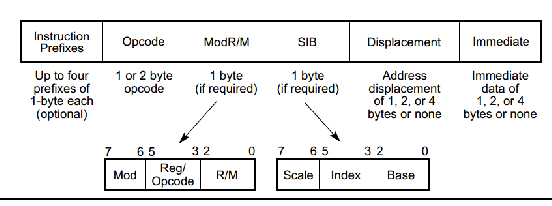
\includegraphics{8086Format_cropped.pdf} 
	\caption{Formatting of Intel 8086 \cite{ref}{8086:ISRef}}
	\label{fig:8086Format}
\end{figure}

\section{Conclusion}
Implementation of a microprocessor design based on a RISC processor will produce an ISA which has good orthogonality with easy decoding. However ,with only a small number of instructions to be implemented to aid simplicity, there is going to be a lot of unused values for the instruction binary. By adding some CISC-style functionality, such as stack operations, density can be improved by incorporating common sequences into one instruction.

It was decided to base an ISA design on the 16-bit ARM Thumb subset. This was because it is an accumulation of the most common instructions from the main ARM ISA and designed to reduce the overall program size compared to its 32-bit counterpart \cite{ref}{ARM:ARM11RefMan}. This means an inherently dense coding, with a wide range of simple instructions. Also, the earlier mentioned investigation at Cornell University suggests there is little difference in terms of code density if there is no 'zero' register like in the ARM \cite{ref}{Density:Correlation}.

\vspace*{\baselineskip}
Word Count: 1686%Manually insert word count, or use online tool/script

%References - Cited references
\newpage
\bibliography{ref}{references}{References}

%Biliography - Non-cited information soruces
%enable internal macro changes, and redefine labelling for bibliography
\makeatletter 
	\renewcommand\@biblabel[1]{\textbullet}
\makeatother
\bibliography{bibl}{bibliography}{Bibliography}
\end{document}

%Removed bibliography entries
%@misc{BIM:HybridRISC,
%	author	= "Iain Mcnally",
%	title	= "Example RISC",
%	howpublished = "",
%	note	= "url: {https://secure.ecs.soton.ac.uk/notes/ bim/notes/fcde/assign/pdf/superrisc.pdf} last viewed on 15/02/2014"
%}
%@misc{Wiki:DLNMOS,
%	author	= "Wikipedia",
%	title	= "Depletion-load NMOS logic",
%	howpublished = "",
%	note	= "url: {http://en.wikipedia.org/ wiki/Depletion-load NMOS logic} last viewed on 15/02/2014"
%}